\documentclass[11pt, a4paper]{article}

\usepackage[utf8]{inputenc}
\usepackage[T1]{fontenc}
\usepackage{lmodern}
\usepackage[margin=2.4cm]{geometry}
\usepackage{microtype}
\usepackage{graphicx}
\usepackage{booktabs}
\usepackage{array}
\usepackage{multirow}
\usepackage{makecell}
\usepackage{caption}
\usepackage{subcaption}
\usepackage{xcolor}
\usepackage{titlesec}
\usepackage{enumitem}
\usepackage{amsmath, amssymb}
\usepackage{hyperref}
\hypersetup{
  colorlinks=true,
  linkcolor=black,
  citecolor=blue!50!black,
  urlcolor=blue!50!black,
}
\usepackage{fancyhdr}
\usepackage{siunitx}
\sisetup{detect-all, table-format=1.4}

\pagestyle{fancy}
\fancyhf{}
\rhead{\small FEELIN Phase 1 Wrap-up Report}
\lhead{\small 2026-05-27}
\rfoot{\thepage}

\titleformat{\section}{\large\bfseries}{\thesection}{0.6em}{}
\titleformat{\subsection}{\normalsize\bfseries}{\thesubsection}{0.5em}{}

\setlength{\parskip}{6pt}
\setlength{\parindent}{0pt}

\newcommand{\fefn}[1]{\texttt{\small #1}}
\newcommand{\eg}{e.g.,\ }
\newcommand{\ie}{i.e.,\ }

\title{\vspace{-2em}\textbf{A Frozen-Probe Benchmark for Brain Foundation Models on
       Naturalistic Emotion fMRI}}
\author{Seokjin Moon \\
        \small Department of Brain and Cognitive Sciences, Seoul National University}
\date{2026-05-27}

\begin{document}
\maketitle
\thispagestyle{fancy}

\begin{abstract}
\noindent
Brain foundation models (BFMs) pretrained on large-scale functional MRI (fMRI) are
increasingly used as frozen feature extractors for downstream cognitive and clinical
tasks. Their behaviour on naturalistic emotional experience, a stimulus-locked regime
distant from the resting-state objective of their pretraining, has not yet been evaluated
under a unified protocol. We introduce a frozen-probe benchmark on the Horikawa
naturalistic emotion fMRI dataset (5 subjects, 2185 short video clips) that places three
published BFMs (SwiFT, Brain-JEPA, NeuroSTORM) against a 450-region atlas baseline and a
video stimulus-feature ceiling drawn from five pretrained vision and vision-language
models. All systems are evaluated under a single 5-fold stimulus-stratified
cross-validation protocol on four emotion tasks (valence and arousal, each as
quartile-extreme classification and continuous regression), with both linear and MLP
probe heads and both pooled and per-subject training modes. A controlled five-way
temporal-padding ablation on SwiFT additionally characterises the contribution of
temporal context to frozen brain embeddings. The benchmark provides a reproducible
reference for the emerging class of joint fMRI-video integration models and surfaces
methodological constraints (pretrain-target domain mismatch, padding dominance under
heavy temporal sparsity, and the limited use of temporal context by frozen probes) that
future work in this regime will need to address.
\end{abstract}

\section{Introduction}

The past two years have produced a growing family of brain foundation models (BFMs) that
treat fMRI as a sequence amenable to self-supervised pretraining at scale. Three
representative examples (SwiFT, Brain-JEPA, NeuroSTORM) pretrain on hundreds of thousands
of resting-state scans from UK Biobank or ABCD, and each has been promoted as a general
purpose feature extractor for downstream cognitive and clinical tasks. Adoption of these
models in practice, however, faces an empirical gap. Their downstream behaviour has been
characterised mostly on phenotype prediction (age, sex, IQ) and short-window classification
tasks aligned with the resting-state regime of pretraining. \emph{Naturalistic emotion
fMRI}, in which subjects view short video clips and the goal is to recover an evoked
affective response, sits in a regime distant from this validation set. The temporal length
of each evoked response is short (5 to 15 TR) relative to the fixed-length input of every
BFM (typically 20 TR), so the majority of the input slots must be filled by padding, and
the signal of interest is stimulus-locked rather than spontaneous. Whether the
representations learned by these BFMs transfer to this regime, and whether the choice of
BFM matters compared to simpler baselines, has not yet been answered under a single,
controlled protocol.

A second motivation comes from the multimodal nature of naturalistic emotion fMRI. The
same stimulus that elicits the brain response is itself a video clip whose affective
content can be recovered, in principle, from pretrained vision models alone (CLIP,
DINOv2, V-JEPA2, VideoMAE) or from automatic captioning. For any future model that
combines brain and video as joint inputs, it is essential to know in advance how much of
the predictable variance is attributable to the stimulus video versus to the brain
response. Without this decomposition, an apparently strong joint model could simply be
re-discovering the stimulus signal that any vision encoder already provides.

This paper provides the missing reference. We benchmark three BFMs, a 450-region atlas
baseline, and five pretrained video models on the same naturalistic emotion fMRI dataset
(Horikawa, 5 subjects across 2185 short clips), under a single 5-fold
stimulus-stratified cross-validation protocol across four emotion tasks. Our specific
contributions are as follows.

\begin{enumerate}[leftmargin=1.4em, itemsep=2pt]
  \item A reproducible cross-model comparison of three frozen BFMs on naturalistic
        emotion fMRI under a single evaluation protocol, with both a simple statistical
        floor (ROI mean BOLD) and a stimulus-only ceiling (pretrained video features) for
        context.
  \item A controlled temporal-padding ablation on SwiFT (five padding modes across four
        tasks), characterising how the short stimulus length and the resulting heavy
        padding shape frozen-embedding behaviour.
  \item A methodological note (\S\,\ref{sec:bjnote}) on the input-length configuration of
        Brain-JEPA, whose flexible patch design admits a different and arguably more
        defensible default than the SwiFT and NeuroSTORM convention; we report all
        Brain-JEPA numbers under the revised configuration.
\end{enumerate}

This report covers the four valence and arousal tasks. Two additional tasks (Cowen-34
categorical classification and Cowen-14 dimensional regression) were extracted in the
underlying CSVs and are released as supplementary material but are not the focus here.

\section{Methods}

\subsection{Dataset and stimuli}
We use the Horikawa naturalistic emotion fMRI corpus, comprising five subjects who viewed
2185 short video clips during 3T fMRI scanning. Each clip is associated with self-rated
valence and arousal (continuous, $[1, 5]$) and Cowen-style category and dimension labels.
The temporal length of each stimulus presentation is 5 to 15~TR, with 71.6\% of stimuli at
$T = 5$. We use the canonical 2185-stimulus index
(\fefn{data/feelin\_canonical\_stimuli.csv}) throughout.

\subsection{Tasks and targets}
Four emotion tasks are evaluated. The two binary tasks restrict the dataset to extreme
quartiles (Q4 vs.\ Q1 of valence or arousal), discarding the middle 50\% to avoid label
boundary noise. The regression tasks use all 2185 stimuli with the continuous rating as
target. Table~\ref{tab:tasks} summarises the formal definitions.

\begin{table}[h]
\centering
\caption{Emotion tasks evaluated. $N_{\text{stim}}$ is the count of stimuli passing the
inclusion filter (binary tasks restrict to extreme quartiles).}
\label{tab:tasks}
\small
\begin{tabular}{lllc}
\toprule
Task & Type & Main metric & $N_{\text{stim}}$ \\
\midrule
V\_binary    & binary (extreme Q4 vs Q1 of valence)         & AUROC      & 1135 \\
A\_binary    & binary (extreme Q4 vs Q1 of arousal)         & AUROC      & 1135 \\
V\_reg       & continuous regression (valence rating)       & Pearson $r$ + MAE + MSE & 2185 \\
A\_reg       & continuous regression (arousal rating)       & Pearson $r$ + MAE + MSE & 2185 \\
\bottomrule
\end{tabular}
\end{table}

\subsection{Models evaluated}
\label{sec:models}

\paragraph{Tier 0 (chance).} For each task, dummy predictors provide an absolute floor.
For binary tasks we report \texttt{most\_frequent} (deterministic majority) and
\texttt{stratified} (random with marginal label distribution, three seeds). For regression
we report \texttt{mean} and \texttt{median} predictors. The chance baseline uses sklearn
dummy estimators only; it is included to anchor every other number in the report.

\paragraph{Tier 1 (statistical floor).} The cortical parcellation Schaefer 17networks 400
combined with the subcortical Tian S3 50 yields a 450-region atlas. For each stimulus, the
ROI BOLD time series is averaged across time to produce a 450-dimensional feature vector.
This feature is the simplest possible representation that respects coarse anatomical
boundaries without learned temporal dynamics.

\paragraph{Tier 2 (brain foundation models).} Three pretrained BFMs are extracted with
both their original pretrained weights (\texttt{resting}) and randomly initialised
weights (\texttt{scratch}) as an architecture-only control.

\begin{itemize}[leftmargin=1.4em, itemsep=2pt]
  \item \textbf{SwiFT NewE96} (ver11, $d_{\text{embed}}=96$, patch $[6,6,6,1]$).
        4D Swin Transformer pretrained at sequence length 20 on UKB and ABCD resting-state
        fMRI. Architecturally locked to $T=20$. Output dimension 768.
  \item \textbf{Brain-JEPA} (ViT-Base, patch 16 in time). Treats input as a
        $(450 \times T)$ image with per-ROI temporal patches of size $(1, 16)$. Variable
        $T$ is supported via positional-embedding resizing. Pretrained on UKB resting-state
        with crop $(450, 160)$, that is, ten time patches per ROI. Output dimension 768.
  \item \textbf{NeuroSTORM} (Swin-UNETR-style 4D). MAE-pretrained on ABCD at
        \texttt{img\_size}$=(96, 96, 96, 20)$. Patch $(6, 6, 6, 1)$. Output dimension 288.
\end{itemize}

\paragraph{Tier 3 (video stimulus features).} Five pretrained video encoders provide a
stimulus-prediction ceiling. Each is also evaluated in a randomly-initialised
\texttt{\_scratch} variant as an architecture-only control.

\begin{itemize}[leftmargin=1.4em, itemsep=2pt]
  \item \textbf{V-JEPA2}: pretrained on large-scale natural video.
  \item \textbf{CLIP}: pretrained on web image and text pairs.
  \item \textbf{DINOv2}: self-supervised pretraining on web-scale images.
  \item \textbf{VideoMAE}: masked-autoencoder pretraining on Kinetics.
  \item \textbf{Qwen-VL caption}: text embedding of automatic emotion-relevant captions
        produced by a vision-language model.
\end{itemize}

\subsection{Padding for variable-length stimuli}
\label{sec:padding}

All three BFMs require a fixed-length 20-TR input. With 71.6\% of stimuli at $T=5$, the
choice of padding fills the unobserved 11 of 16 (Brain-JEPA, after centre cropping) or
15 of 20 (SwiFT, NeuroSTORM) slots. Five padding modes are defined.

\begin{itemize}[leftmargin=1.4em, itemsep=2pt]
  \item \texttt{replicate}: pad with copies of the last observed frame.
  \item \texttt{zero}: pad with zeros.
  \item \texttt{mean}: pad with the per-ROI mean across the observed $T$ frames (proper
        mean padding).
  \item \texttt{spatial\_only}: replace every output frame with the per-ROI mean. This is
        a no-temporal-information control.
  \item \texttt{cyclic\_replicate}: tile the observed frames in a loop, for example
        $(f_0, f_1, f_2, f_3, f_4, f_0, f_1, \dots)$.
\end{itemize}

\paragraph{Default choice: \texttt{zero}.}
We adopt \texttt{zero} as the default padding for all three BFMs in the main grid. The
rationale is alignment with the input scaling convention shared by all three pretrained
models. SwiFT, Brain-JEPA, and NeuroSTORM are all pretrained with the
\texttt{znorm\_minback} input normalisation (z-score with the spatial background set to
zero), and SwiFT and NeuroSTORM additionally apply background-zero \emph{spatial} padding
to reach their fixed $96 \times 96 \times 96$ input size. Under this convention,
zero-valued frames are the natural distributional extension to the time axis: they sit at
the mean of the per-ROI BOLD distribution that the pretrained models were exposed to, and
they do not inject any signal not already present at training time.

For SwiFT we extract embeddings under all five padding modes as a controlled ablation
(\S\,\ref{sec:padding-ablation}) to verify that this default choice does not materially
affect frozen-probe results. For Brain-JEPA and NeuroSTORM, only \texttt{zero} is
extracted for the main grid: Brain-JEPA's per-ROI temporal conv kernel averages within a
16-TR window anyway, and NeuroSTORM was expected to behave similarly to SwiFT (the
SwiFT ablation result, in which \texttt{zero}, \texttt{mean}, \texttt{spatial\_only}, and
\texttt{cyclic\_replicate} are within 0.001 of each other on the overall main metric,
supports treating these four modes as interchangeable for the frozen-probe regime).

\subsection{Brain-JEPA configuration}
\label{sec:bjnote}

Brain-JEPA's per-ROI temporal patch size is 16. Setting \texttt{NUM\_FRAMES}$=$20 (as used
for SwiFT and NeuroSTORM) discards the last 4 TR of every stimulus because the patch
stride is 16. We instead set \texttt{NUM\_FRAMES}$=$16 for Brain-JEPA and apply a
symmetric centre crop for $T \geq 16$ stimuli (drop $\lfloor (T-16)/2 \rfloor$ TR from
each end). For $T < 16$ we pad with \texttt{mean}. This change avoids using the initial
hemodynamic transient and discards the last 4 TR symmetrically rather than only at the
end. The legacy extraction (with \texttt{NUM\_FRAMES}$=$20 and first-16 cropping) is
archived as \fefn{output/embeddings/brain\_jepa\_LEGACY\_T20first16\_*}.

\subsection{Probe heads}
For every feature vector and every task, two probe heads are trained on the training fold.

\begin{itemize}[leftmargin=1.4em, itemsep=2pt]
  \item \textbf{Linear}: deterministic ridge regression (continuous tasks) or logistic
        regression (binary). Regularisation strength is selected from
        $\{10^{-3}, 10^{-2}, \ldots, 10^{2}\}$ on the validation fold. Since the linear
        solver is deterministic, a single seed (0) is used.
  \item \textbf{MLP}: two residual blocks with hidden dimension 256, GELU activation,
        dropout 0.3. The learning rate is selected from
        $\{10^{-4}, 3\!\cdot\!10^{-4}, \ldots, 10^{-2}\}$ on the validation fold. The
        single seed used here, 0, gives a snapshot estimate. Final-paper runs will use
        three seeds.
\end{itemize}

\subsection{Evaluation protocol}
We use 5-fold stimulus-stratified cross-validation. Stimuli are stratified jointly by
valence quartile and arousal quartile, ensuring that every fold has comparable distribution
of extreme stimuli. The exact split is fixed as \fefn{data/horikawa\_5fold.csv}
(\texttt{random\_state}$=$0). For each outer fold $k$ we use fold $k$ as test, fold
$((k \bmod 5) + 1)$ as validation, and the remaining three folds as training. For BFM and
ROI features we additionally distinguish two evaluation modes: \texttt{pooled} (all five
subjects merged into a single training set, one fit per fold) and \texttt{per\_subject}
(one fit per subject, five fits per fold, reported as the mean over subjects). Video
features are subject-independent and use a single \texttt{stim\_level} mode.

\subsection{Reproducibility}
All evaluation CSVs include per-fold rows; aggregation to mean $\pm$ std is performed by
\fefn{code/probes/\_summary\_helper.py}. The benchmark tables in this report are generated
by \fefn{code/analysis/phase1\_benchmark\_table.py}. Figures are produced by
\fefn{code/analysis/phase1\_unified\_analysis.py}.

\clearpage

\section{Main results}

\subsection{Per-task ranking}

Tables~\ref{tab:vbinary} to \ref{tab:areg} summarise the top entries per task. Two
consistent patterns appear immediately. (i) Pretrained video features dominate every task
by a wide margin. (ii) Within the brain-input category, the simple
Schaefer-400+Tian-50 ROI mean baseline outperforms every frozen BFM.

\paragraph{Interpretation.}
The brain-to-video gap is large enough to constitute a clear floor that Phase 2 trained
integration must close. On valence-binary the gap is $+0.18$ AUROC, on arousal-binary
$+0.13$ AUROC; on the continuous tasks the gap is $+0.35$ (V\_reg) and $+0.19$ (A\_reg) in
Pearson $r$, with MAE differences of $0.44$ on V\_reg and effectively zero on A\_reg.
That CLIP, an image-text model never trained on emotion data nor on brain data, can
predict a brain-mediated emotion label so much better than every brain encoder is direct
evidence that the stimulus video carries the dominant signal for this evaluation, and that
frozen brain embeddings recover only a small fraction of it.

\begin{table}[h]
\centering
\caption{V\_binary (AUROC). Top 5 of each category. Mean $\pm$ standard deviation across
the 5-fold CV; for \texttt{per\_subject} mode, additionally averaged across 5 subjects
(n=25). Chance is $0.500$ (deterministic majority).}
\label{tab:vbinary}
\small
\setlength{\tabcolsep}{4pt}
\begin{tabular}{rlllllS[table-format=1.4]S[table-format=1.4]}
\toprule
\# & Feature & Init & Padding & Head & Mode & {AUROC $\mu$} & {AUROC $\sigma$} \\
\midrule
\multicolumn{8}{l}{\textit{Brain models (chance = 0.5000, fMRI input)}} \\
1 & ROI\_Schaefer400Tian50 & n/a     & time\_mean & linear & pooled       & \bfseries 0.7889 & 0.0119 \\
2 & ROI\_Schaefer400Tian50 & n/a     & time\_mean & linear & per\_subject & 0.7885 & 0.0263 \\
3 & ROI\_Schaefer400Tian50 & n/a     & time\_mean & mlp    & pooled       & 0.7626 & 0.0142 \\
4 & ROI\_Schaefer400Tian50 & n/a     & time\_mean & mlp    & per\_subject & 0.7601 & 0.0319 \\
5 & NeuroSTORM             & resting & mean       & linear & per\_subject & 0.7292 & 0.0361 \\
\midrule
\multicolumn{8}{l}{\textit{Video models (stimulus-feature input)}} \\
1 & CLIP\_pretrained      & n/a & n/a & linear & stim\_level & \bfseries 0.9708 & 0.0112 \\
2 & CLIP\_pretrained      & n/a & n/a & mlp    & stim\_level & 0.9520 & 0.0078 \\
3 & DINOv2\_pretrained    & n/a & n/a & linear & stim\_level & 0.9135 & 0.0071 \\
4 & Qwen-VL\_caption      & n/a & n/a & linear & stim\_level & 0.9024 & 0.0165 \\
5 & DINOv2\_pretrained    & n/a & n/a & mlp    & stim\_level & 0.8814 & 0.0078 \\
\bottomrule
\end{tabular}
\end{table}

\paragraph{Conclusion for V\_binary.}
The brain ceiling (\num{0.789}) is well above chance but $0.182$ AUROC below the video
ceiling (\num{0.971}). CLIP achieves \num{0.971}, indicating that for valence-extreme
discrimination the stimulus itself is highly informative even without any brain signal.

\begin{table}[h]
\centering
\caption{A\_binary (AUROC). Chance $=0.500$.}
\label{tab:abinary}
\small
\setlength{\tabcolsep}{4pt}
\begin{tabular}{rlllllS[table-format=1.4]S[table-format=1.4]}
\toprule
\# & Feature & Init & Padding & Head & Mode & {AUROC $\mu$} & {AUROC $\sigma$} \\
\midrule
\multicolumn{8}{l}{\textit{Brain models}} \\
1 & ROI\_Schaefer400Tian50 & n/a     & time\_mean & linear & pooled       & \bfseries 0.6784 & 0.0532 \\
2 & ROI\_Schaefer400Tian50 & n/a     & time\_mean & linear & per\_subject & 0.6694 & 0.0437 \\
3 & ROI\_Schaefer400Tian50 & n/a     & time\_mean & mlp    & pooled       & 0.6595 & 0.0388 \\
4 & Brain-JEPA             & resting & mean       & linear & pooled       & 0.6486 & 0.0324 \\
5 & Brain-JEPA             & scratch & mean       & linear & pooled       & 0.6407 & 0.0397 \\
\midrule
\multicolumn{8}{l}{\textit{Video models}} \\
1 & CLIP\_pretrained       & n/a & n/a & linear & stim\_level & \bfseries 0.8003 & 0.0521 \\
2 & CLIP\_pretrained       & n/a & n/a & mlp    & stim\_level & 0.7813 & 0.0401 \\
3 & VideoMAE\_pretrained   & n/a & n/a & linear & stim\_level & 0.7465 & 0.0196 \\
4 & V-JEPA2\_pretrained    & n/a & n/a & linear & stim\_level & 0.7339 & 0.0380 \\
5 & DINOv2\_pretrained     & n/a & n/a & linear & stim\_level & 0.7278 & 0.0603 \\
\bottomrule
\end{tabular}
\end{table}

\paragraph{Conclusion for A\_binary.}
Arousal-extreme is harder to decode than valence-extreme for every model. Both ceilings
drop substantially compared to V\_binary (best brain \num{0.678} vs.\ \num{0.789}; best
video \num{0.800} vs.\ \num{0.971}). The brain-video gap narrows to $+0.122$ AUROC.
This is consistent with the standard finding that arousal is harder to predict from
both visual stimuli and brain signals than valence in naturalistic settings.

\begin{table}[h]
\centering
\caption{V\_reg (continuous valence regression). Top 5 of each category. Pearson $r$ is
the main metric (higher is better); MAE and MSE are also reported for completeness (lower
is better). Chance for $r$ is $0.000$ (constant predictor has undefined correlation,
taken as zero).}
\label{tab:vreg}
\small
\setlength{\tabcolsep}{3.5pt}
\begin{tabular}{rlllllS[table-format=1.4]S[table-format=1.4]S[table-format=1.4]S[table-format=1.4]}
\toprule
\# & Feature & Init & Padding & Head & Mode & {$r$ $\mu$} & {$r$ $\sigma$} & {MAE $\mu$} & {MSE $\mu$} \\
\midrule
\multicolumn{10}{l}{\textit{Brain models}} \\
1 & ROI\_Schaefer400Tian50 & n/a     & time\_mean & mlp    & pooled       & \bfseries 0.4158 & 0.0220 & \bfseries 1.4870 & 3.4119 \\
2 & ROI\_Schaefer400Tian50 & n/a     & time\_mean & linear & per\_subject & 0.4042 & 0.0310 & 1.4963 & 3.3132 \\
3 & ROI\_Schaefer400Tian50 & n/a     & time\_mean & mlp    & per\_subject & 0.4024 & 0.0446 & 1.5619 & 3.8856 \\
4 & ROI\_Schaefer400Tian50 & n/a     & time\_mean & linear & pooled       & 0.3964 & 0.0131 & 1.4991 & \bfseries 3.2920 \\
5 & NeuroSTORM             & resting & mean       & linear & per\_subject & 0.3119 & 0.0471 & 1.5696 & 3.5814 \\
\midrule
\multicolumn{10}{l}{\textit{Video models}} \\
1 & CLIP\_pretrained       & n/a & n/a & mlp    & stim\_level & \bfseries 0.7645 & 0.0309 & \bfseries 1.0446 & \bfseries 1.8286 \\
2 & CLIP\_pretrained       & n/a & n/a & linear & stim\_level & 0.6832 & 0.0243 & 1.2011 & 2.3084 \\
3 & DINOv2\_pretrained     & n/a & n/a & mlp    & stim\_level & 0.6008 & 0.0360 & 1.3958 & 3.1539 \\
4 & Qwen-VL\_caption       & n/a & n/a & mlp    & stim\_level & 0.5990 & 0.0395 & 1.3723 & 3.1159 \\
5 & Qwen-VL\_caption       & n/a & n/a & linear & stim\_level & 0.5741 & 0.0263 & 1.3189 & 2.7260 \\
\bottomrule
\end{tabular}
\end{table}

\paragraph{Conclusion for V\_reg.}
CLIP plus MLP reaches Pearson $r=\num{0.765}$ with MAE \num{1.045}, while the best brain
configuration (ROI plus MLP, pooled) reaches $r=\num{0.416}$ with MAE \num{1.487}. The
brain ceiling captures only about one-third of the variance that video features
explain ($r^2$: \num{0.17} vs.\ \num{0.58}). The MAE gap of $0.44$ rating units is
practically large given a $[1,5]$ rating scale.

\begin{table}[h]
\centering
\caption{A\_reg (continuous arousal regression). MAE and MSE included.}
\label{tab:areg}
\small
\setlength{\tabcolsep}{3.5pt}
\begin{tabular}{rlllllS[table-format=1.4]S[table-format=1.4]S[table-format=1.4]S[table-format=1.4]}
\toprule
\# & Feature & Init & Padding & Head & Mode & {$r$ $\mu$} & {$r$ $\sigma$} & {MAE $\mu$} & {MSE $\mu$} \\
\midrule
\multicolumn{10}{l}{\textit{Brain models}} \\
1 & ROI\_Schaefer400Tian50 & n/a     & time\_mean & linear & pooled       & \bfseries 0.2334 & 0.0524 & \bfseries 0.7120 & \bfseries 0.8061 \\
2 & ROI\_Schaefer400Tian50 & n/a     & time\_mean & mlp    & pooled       & 0.2254 & 0.0497 & 0.7328 & 0.8544 \\
3 & ROI\_Schaefer400Tian50 & n/a     & time\_mean & linear & per\_subject & 0.2207 & 0.0576 & 0.7232 & 0.8364 \\
4 & Brain-JEPA             & resting & mean       & linear & pooled       & 0.2064 & 0.0306 & 0.7130 & 0.8064 \\
5 & ROI\_Schaefer400Tian50 & n/a     & time\_mean & mlp    & per\_subject & 0.2003 & 0.0567 & 0.7641 & 0.9426 \\
\midrule
\multicolumn{10}{l}{\textit{Video models}} \\
1 & CLIP\_pretrained       & n/a & n/a & mlp    & stim\_level & \bfseries 0.4231 & 0.0421 & \bfseries 0.7133 & \bfseries 0.7998 \\
2 & CLIP\_pretrained       & n/a & n/a & linear & stim\_level & 0.3375 & 0.0472 & 0.7787 & 0.9634 \\
3 & V-JEPA2\_pretrained    & n/a & n/a & mlp    & stim\_level & 0.3237 & 0.0567 & 0.8019 & 1.0246 \\
4 & VideoMAE\_pretrained   & n/a & n/a & mlp    & stim\_level & 0.3043 & 0.0307 & 0.7981 & 1.0090 \\
5 & Qwen-VL\_caption       & n/a & n/a & mlp    & stim\_level & 0.3013 & 0.0287 & 0.7193 & 0.8447 \\
\bottomrule
\end{tabular}
\end{table}

\paragraph{Conclusion for A\_reg.}
Arousal regression is the hardest task in the benchmark. The best Pearson $r$ across all
models is only \num{0.423} (CLIP plus MLP), and the best brain configuration reaches
\num{0.233}. Notably, on MAE the gap between brain best (\num{0.712}) and video best
(\num{0.713}) is essentially zero, even though Pearson $r$ favours video by \num{0.19}.
This means video predictions track the rank ordering of arousal better than brain
predictions, but in absolute error both are similar. For binary or rank-based downstream
use the video advantage is real; for absolute-magnitude use it is negligible.

\subsection{Visual summary of per-task ranking}

Figure~\ref{fig:ranking} shows the full per-task best-condition ranking across all feature
classes. The video category occupies the upper portion of every plot, with the ROI floor
sitting at the top of the brain category. Numerical mean and $\pm$standard deviation are
annotated directly above each bar.

\begin{figure}[h]
\centering
\begin{subfigure}{0.49\textwidth}
\includegraphics[width=\linewidth]{figs/ranking_V_binary.png}\caption{V\_binary}\end{subfigure}\hfill
\begin{subfigure}{0.49\textwidth}
\includegraphics[width=\linewidth]{figs/ranking_A_binary.png}\caption{A\_binary}\end{subfigure}\\[4pt]
\begin{subfigure}{0.49\textwidth}
\includegraphics[width=\linewidth]{figs/ranking_V_reg.png}\caption{V\_reg}\end{subfigure}\hfill
\begin{subfigure}{0.49\textwidth}
\includegraphics[width=\linewidth]{figs/ranking_A_reg.png}\caption{A\_reg}\end{subfigure}
\caption{Best condition per (feature, init) on each task. Bars show mean across 5 folds;
error bars are the within-fold standard deviation. Bar labels report mean above
($\pm$std). Grey dashed lines mark the deterministic chance baseline. Brain features (blue
family) cluster below video pretrained features (orange) on every task, with the ROI
baseline (light blue) consistently above the three BFMs.}
\label{fig:ranking}
\end{figure}

\paragraph{What the four panels show together.}
Panel (a) and (b) (the two binary tasks) reveal the same qualitative ordering. Video
pretrained features cluster at the top, video scratch features fall to the bottom of the
video group, and ROI sits at the top of the brain group with BFMs below. Panel (c) and (d)
(the regression tasks) show the same ordering but with a smaller absolute range and with
A\_reg uniformly difficult for all models. The robustness of this ordering across all four
tasks is itself an important result; it implies that the relative ranking of feature
families is not task-specific.

\subsection{ROI floor outperforms frozen BFMs}

Across all four tasks, the simple Schaefer-400 plus Tian-S3-50 ROI mean BOLD probe is the
single best brain-side feature. The advantage over the best BFM ranges from $+0.062$
AUROC (V\_binary: ROI \num{0.789} vs.\ NeuroSTORM \num{0.729}) to $+0.104$ Pearson $r$
(V\_reg: ROI \num{0.416} vs.\ NeuroSTORM \num{0.312}). This pattern persists across both
probe heads, both training modes, and both initialisations. Three plausible contributors
are listed below.

\begin{enumerate}[leftmargin=1.4em, itemsep=1pt]
  \item BFM pretrain task mismatch (resting-state self-supervised objectives vs.\
        stimulus-locked evoked response in our test data).
  \item Small-$N$ regression bias. 768-dimensional BFM features overfit more easily than
        450-dimensional ROI features under ridge regularisation, when only about $1100$
        training stimuli per fold are available.
  \item Padding dominance. 71.6\% of stimuli have $T = 5$, so 11 to 15 of the available
        16 to 20 temporal patch slots are filled with non-evoked content, which the BFM
        Transformer propagates into the embedding.
\end{enumerate}

\paragraph{Practical conclusion.}
The frozen probe of any current BFM is, on this benchmark, dominated by a simple
parcel-wise temporal mean. This does not imply that the BFMs are useless. It implies that
their value, if any, must emerge during \emph{trained} downstream use (\eg fine-tuning,
joint-training as in Phase 2), not from frozen embedding extraction.

\subsection{SwiFT padding ablation: temporal information is not used}
\label{sec:padding-ablation}

Table~\ref{tab:padding} reports the SwiFT NewE96 frozen-embedding performance under all
five padding modes, averaged over initialisation, head, and mode. The result is striking
in its uniformity. The four non-last-frame padding modes are statistically
indistinguishable. \texttt{spatial\_only}, \texttt{mean}, \texttt{zero}, and
\texttt{cyclic\_replicate} differ by at most $0.007$ in overall mean main metric. Only
\texttt{replicate} is materially worse ($\Delta \approx -0.03$).

\begin{table}[h]
\centering
\caption{SwiFT NewE96 padding ablation. Main-metric mean across init, head, mode, fold,
and subject for each task. The rightmost column is the average across tasks. Rows are
sorted by overall mean.}
\label{tab:padding}
\small
\begin{tabular}{lS[table-format=1.4]S[table-format=1.4]S[table-format=1.4]S[table-format=1.4]S[table-format=1.4]}
\toprule
Padding & {A\_binary} & {A\_reg} & {V\_binary} & {V\_reg} & {Overall} \\
\midrule
spatial\_only      & 0.5756 & 0.0993 & 0.6334 & 0.1938 & \bfseries 0.3755 \\
mean               & 0.5731 & 0.0927 & \bfseries 0.6393 & \bfseries 0.1964 & 0.3754 \\
zero               & \bfseries 0.5779 & \bfseries 0.1041 & 0.6328 & 0.1865 & 0.3753 \\
cyclic\_replicate  & 0.5622 & 0.0836 & 0.6359 & 0.1927 & 0.3686 \\
replicate          & 0.5415 & 0.0621 & 0.6169 & 0.1562 & 0.3442 \\
\bottomrule
\end{tabular}
\end{table}

\paragraph{Conclusion for padding.}
The fact that \texttt{spatial\_only} (every padded frame replaced by the per-ROI temporal
mean, that is, zero temporal information) achieves the same performance as \texttt{mean}
(proper temporal mean padding with the real $T$ frames preserved) is informative. It
implies that SwiFT's frozen embedding does not effectively integrate temporal dynamics on
these short, padded inputs. The frozen probe of SwiFT is essentially picking up a
spatial-pattern code from the temporally averaged BOLD activity. The \texttt{replicate}
mode underperforms not because it carries more information but because it injects a
distortion (last-frame attention bias) that the other four modes do not.

\paragraph{Why this matters.}
If frozen SwiFT does not use the temporal dimension, then any methodological argument that
SwiFT is preferred over a static ROI mean because it captures temporal dynamics is not
supported on the present benchmark. To exploit temporal structure, SwiFT or any other BFM
would need to be fine-tuned, not frozen-probed.

\paragraph{Consistency with prior work.}
This observation is consistent with Sartzetaki et al. (ICLR 2025), who showed across 99
video and image models that temporal modeling drives alignment with early visual brain
regions only when the model is trained end-to-end on a task that requires temporal
processing. Their result was obtained on a separate visual fMRI benchmark (BOLD Moments)
using Representational Similarity Analysis, but the broader claim transfers: temporal
context provides brain-relevant signal in principle, but extracting it requires trained
representations rather than frozen-probe regimes. The present ablation establishes the
analogous frozen-probe negative for naturalistic emotion fMRI.

\begin{figure}[h]
\centering
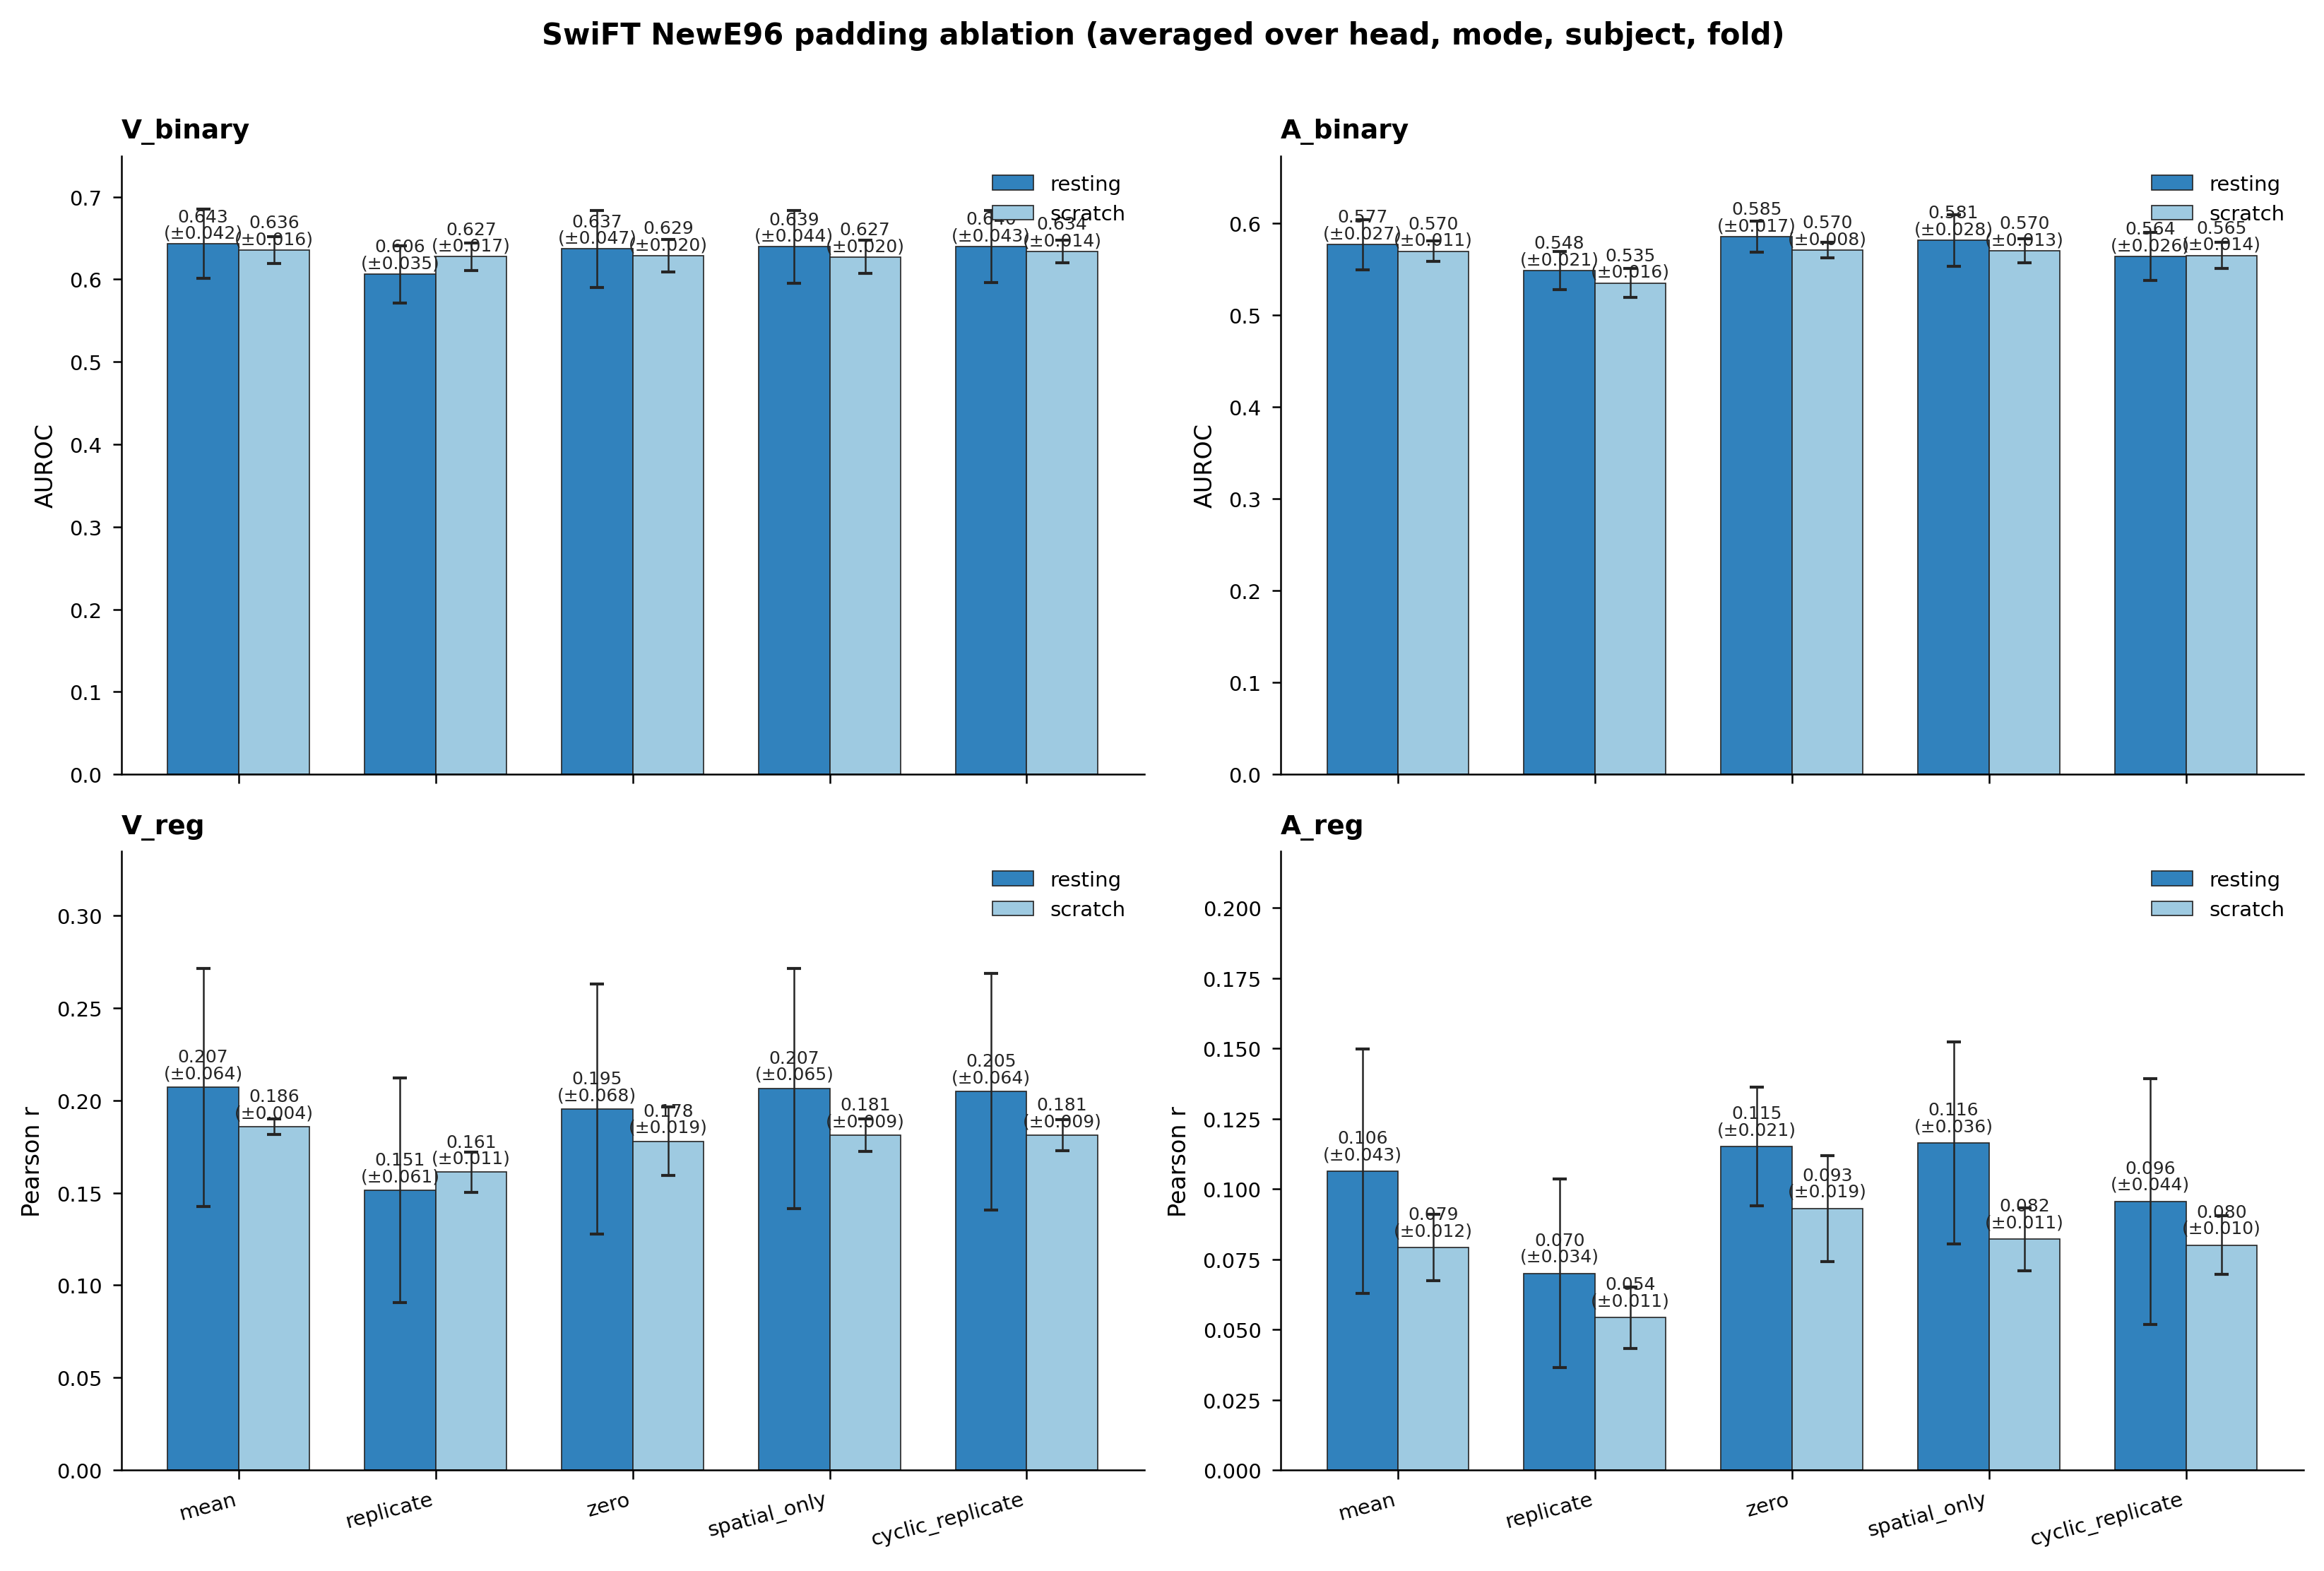
\includegraphics[width=0.95\linewidth]{figs/padding_ablation.png}
\caption{SwiFT NewE96 padding ablation. Bars show mean across head, mode, subject, and
fold; error bars are the standard deviation across folds. Numbers above bars report mean
and $\pm$std. Four padding modes are within fold variance of each other on every task;
only last-frame replicate is consistently worse.}
\label{fig:padding}
\end{figure}

\subsection{Pretraining adds a small but consistent gain (resting vs.\ scratch)}

Across BFMs, the resting-state pretrained initialisation outperforms the random
initialisation by a small but consistent margin: $+0.03$ to $+0.06$ AUROC on the binary
tasks and $+0.03$ to $+0.08$ Pearson $r$ on the regression tasks. This is the weakest
positive finding of the report. Pretraining contributes, but does not transform frozen
embeddings into a feature class competitive with video pretrained features.

\paragraph{Conclusion.}
The fact that random initialisation alone (the \texttt{scratch} variant) already produces
embeddings within \num{0.05} AUROC of the pretrained ones suggests that, on this
benchmark, much of what the frozen BFMs ``do'' is architectural inductive bias rather than
learned representation. The pretraining gain exists but is not the dominant source of
performance.

\subsection{SwiFT model size and architecture variant}
\label{sec:swift-variants}

To test whether SwiFT model size or architecture variant (older \texttt{ver9} UAH series
with temporal patch 2 vs.\ newer \texttt{ver11} NewE series with temporal patch 1) affects
emotion task performance, we extracted embeddings from five additional SwiFT checkpoints
under the main-grid \texttt{zero} padding default, spanning a 50$\times$ range in
parameter count.

\begin{table}[h]
\centering
\caption{SwiFT model variants (best condition per variant per task). Variants are ordered
by parameter count. Reference rows at the bottom show the best brain-side model from the
main grid (ROI, Brain-JEPA, NeuroSTORM). All values are mean across 5 folds. Main metric
is AUROC for binary tasks and Pearson $r$ for regression tasks.}
\label{tab:swift-variants}
\small
\setlength{\tabcolsep}{4pt}
\begin{tabular}{l c S[table-format=1.4] S[table-format=1.4] S[table-format=1.4] S[table-format=1.4]}
\toprule
Variant & params (M) & {V\_binary} & {A\_binary} & {V\_reg} & {A\_reg} \\
\midrule
\multicolumn{6}{l}{\textit{ver9 (UAH series, temporal patch 2)}} \\
UAH\_5M             &   5 & 0.6700 & 0.6015 & 0.2136 & 0.1220 \\
UAH\_51M            &  51 & 0.6660 & 0.6159 & 0.2237 & 0.1414 \\
UAH\_202M           & 202 & \bfseries 0.6911 & \bfseries 0.6206 & \bfseries 0.2636 & 0.1456 \\
\midrule
\multicolumn{6}{l}{\textit{ver11 (NewE series, temporal patch 1)}} \\
NewE36              &   9 & 0.6615 & 0.6130 & 0.2168 & \bfseries 0.1560 \\
NewE96 (main)       &  66 & 0.6884 & 0.6055 & 0.2564 & 0.1414 \\
NewE192             & 264 & 0.6863 & 0.6093 & 0.2552 & 0.1432 \\
\midrule
\multicolumn{6}{l}{\textit{Reference (best brain-side, from main grid)}} \\
NeuroSTORM          &  -- & 0.7292 & 0.6372 & 0.3119 & 0.1911 \\
Brain-JEPA          &  -- & 0.7402 & 0.6624 & 0.3296 & 0.2214 \\
ROI 450             &  -- & \bfseries 0.7889 & \bfseries 0.6784 & \bfseries 0.4158 & \bfseries 0.2334 \\
\bottomrule
\end{tabular}
\end{table}

\paragraph{Three findings.}
First, there is a \emph{modest} size effect within SwiFT on the valence-side tasks. On
V\_binary, the AUROC rises from \num{0.66} at 5M to \num{0.69} at 202M parameters
(+\num{0.02}). On V\_reg, Pearson $r$ rises from \num{0.21} to \num{0.26} (+\num{0.05}).
On the arousal-side tasks (A\_binary, A\_reg), the size effect is statistically
indistinguishable from zero. Second, the older \texttt{ver9} (UAH) and newer \texttt{ver11}
(NewE) families are practically tied at every comparable size point; the temporal-patch-1
NewE family does not yield a measurable advantage. Third, even the largest SwiFT variant
(NewE192 at 264M, or UAH\_202M at 202M) remains \emph{below the Brain-JEPA, NeuroSTORM, and
ROI baselines} on every task. The largest SwiFT model on V\_binary reaches AUROC
\num{0.69}, which is still \num{0.05} below Brain-JEPA, \num{0.04} below NeuroSTORM, and
\num{0.10} below the 450-region ROI mean baseline.

\paragraph{Connection to Sartzetaki et al. (2025).}
Sartzetaki et al.\ reported a negative correlation between model FLOPs and brain alignment
in higher-level visual regions for video models. Our SwiFT variant comparison provides an
analogous \emph{flat} (rather than negative) pattern in the emotion-decoding regime:
within a single architecture family, scaling from 5M to 264M parameters does not improve
frozen-probe emotion performance beyond noise on the arousal tasks and produces only modest
gains on the valence tasks. This is consistent with the broader claim that simply scaling
brain-side parameters under a frozen-probe regime does not recover task-relevant emotion
information.

\paragraph{Conclusion.}
The SwiFT family does not have a missing-size sweet spot for emotion decoding on this
benchmark; every tested SwiFT variant from 5M to 264M parameters underperforms ROI mean
BOLD and the other two BFMs. Selecting one SwiFT variant for Phase 2 fine-tuning should
prioritise architectural and engineering considerations (training stability, memory
budget) rather than expected frozen-probe performance, since the latter is essentially
constant across the size axis.

\subsection{Pooled vs.\ per-subject mode}

For binary tasks the two modes are essentially indistinguishable
($|\Delta| < 0.01$ on V\_binary, $\Delta = +0.012 \pm 0.017$ on A\_binary in favour of
pooled). For regression, pooled has a small but more consistent advantage, particularly on
A\_reg ($\Delta = +0.026 \pm 0.021$).

\paragraph{Conclusion.}
The two modes are practically equivalent on classification, with pooled slightly favoured
on regression. The standard interpretation is that pooling acts as additional implicit
regularisation when single-subject sample sizes are small (about $440$ per subject in the
training fold). For Phase 2 the recommended default is \texttt{pooled}, since it produces
stabler regression numbers without sacrificing classification quality. See
Figure~\ref{fig:mode} for the cell-level comparison.

\begin{figure}[h]
\centering
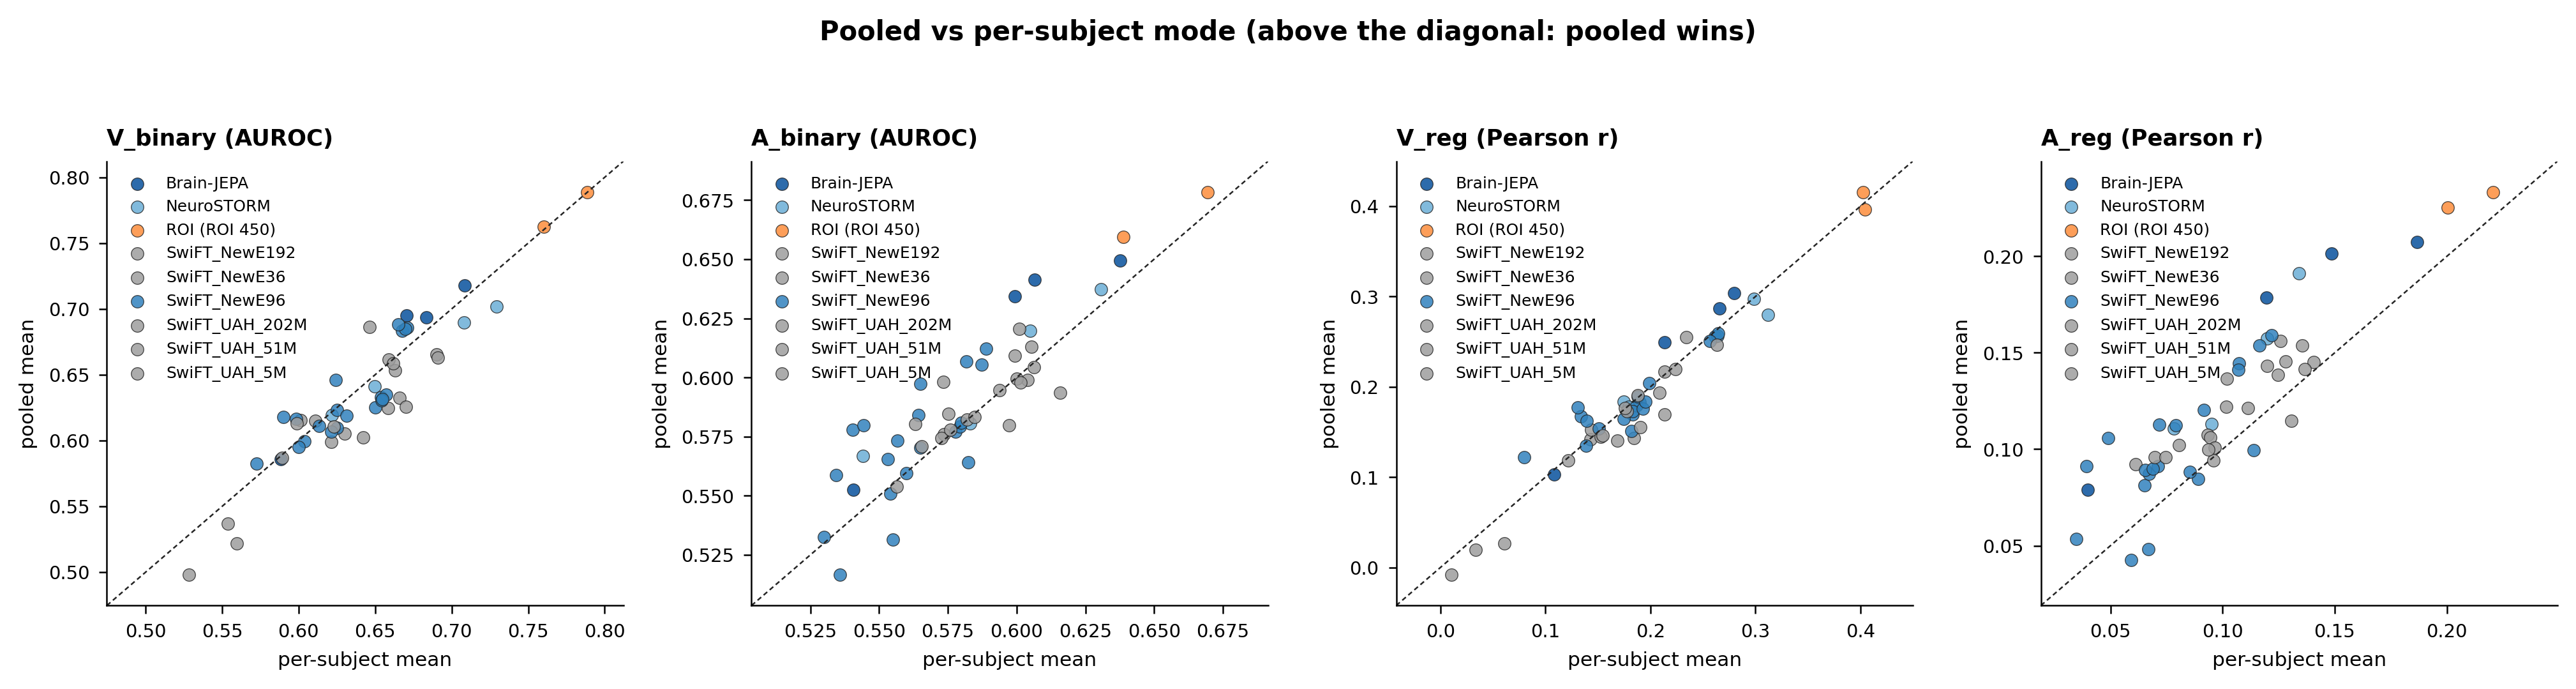
\includegraphics[width=0.95\linewidth]{figs/mode_comparison.png}
\caption{Pooled vs.\ per-subject mode for each (feature, init, padding, head) cell on each
task. Points above the diagonal indicate the pooled mode is better. For regression tasks
(rightmost two panels) the cloud sits modestly above the diagonal, consistent with the
small positive $\Delta$ reported in the main text.}
\label{fig:mode}
\end{figure}

\clearpage

\section{Discussion}

\subsection{What this benchmark establishes}

This Phase 1 report establishes, under a single common protocol, three results.

\begin{enumerate}[leftmargin=1.4em, itemsep=2pt]
  \item The three brain foundation models tested in their frozen state do not yield
        embedding representations of naturalistic emotion fMRI that exceed a 450-region
        mean BOLD ridge baseline.
  \item Pretrained video features set a high stimulus-prediction ceiling that brain
        features fall systematically short of, ranging from $+0.13$ to $+0.18$ AUROC on
        the binary tasks and $+0.19$ to $+0.35$ Pearson $r$ on the regression tasks.
  \item Within the SwiFT frozen probe, no padding strategy that preserves temporal
        information meaningfully outperforms a temporal-mean control, suggesting that the
        frozen SwiFT embedding on these short padded inputs is essentially a spatial
        code.
\end{enumerate}

These three findings together delineate the gap that any trained joint architecture in
Phase 2 must close. The gap is not small, and the contribution of brain information will
need to come either from (a) joint training that exploits brain features the frozen probe
cannot expose, or (b) reframing the evaluation toward subject-specific subjective response
that the video features cannot, in principle, predict.

\subsection{Why ROI beats BFM, in plain terms}

The Schaefer-400 plus Tian-S3-50 mean BOLD vector is a fixed, low-dimensional summary of
the exact same input that the BFMs see. It carries no learned temporal pattern, no learned
spatial inductive bias, and no pretraining-derived prior; only a parcellation. That this
representation outperforms three pretrained Transformer-based BFMs on every task should be
read as evidence that, for stimulus-level emotion prediction under heavy temporal padding,
the BFMs' learned representations are not contributing positive task-relevant information
beyond what raw mean BOLD already provides. The most plausible reason is the combination
of pretraining-test domain mismatch and the 75\% padding ratio that defines our evaluation
set.

\paragraph{This is a frozen-probe statement, not a verdict on the BFMs.}
We want to be precise about what the present results do and do not show. The result is
that the \emph{frozen embeddings} of three resting-state-pretrained BFMs are dominated by
a parcel-wise temporal mean. It is \emph{not} a statement that these BFMs are uninformative
for naturalistic emotion fMRI. Several mechanisms could in principle recover the gap that
frozen probes leave on the table. Among them are end-to-end fine-tuning of the BFM on
emotion targets, parameter-efficient adaptation (\eg LoRA on a subset of layers), and
trained joint architectures that combine the BFM output with a stimulus-side encoder
under a shared loss. The present benchmark establishes that the resting-state
self-supervised pretraining paradigm, when used as a fixed feature extractor under heavy
temporal padding, does not by itself yield representations competitive with simple
parcel-wise summaries. Whether that paradigm can be made competitive by trained downstream
use is an empirical question that Phase 2 is designed to answer.

\subsection{Implications for Phase 2}

The headline take from this benchmark is that the conventional recipe (resting-state
self-supervised pretraining as a feature extractor, frozen probe on downstream emotion
targets) does not transfer to naturalistic emotion fMRI under our protocol. A different
recipe is required, and Phase 2 is positioned to test what that recipe should be. We
identify two non-mutually-exclusive directions.

\begin{enumerate}[leftmargin=1.4em, itemsep=4pt]
  \item \textbf{Replace the frozen probe by trained integration.}
        The frozen-extraction regime discards the largest knob the BFMs have for
        adapting to a new task: their internal parameters. Trained joint architectures
        (LLM-token injection, cross-attention, contrastive alignment, late fusion) all
        provide a path for the BFM representation to be shaped by the emotion target. If
        any of these architectures improves over Tier 3 video features by even a small
        margin, that is the first quantitative demonstration on this benchmark that brain
        features carry information beyond what the stimulus alone provides. Conversely,
        if none does, the negative result is itself informative about the regime.
  \item \textbf{Reframe what brain features are expected to add.}
        Pretrained video models predict the stimulus-level emotion label almost
        perfectly because that label is, by construction, a property of the stimulus.
        Subject-specific subjective experience (the same clip eliciting different
        affective states in different viewers) is not predictable from the video alone
        and is the natural locus of brain contribution. Two concrete operationalisations
        for Phase 2 and 3 are: (a) counterfactual subject swap, in which the same video
        is paired with a different subject's brain response and the resulting model
        output is required to change systematically; (b) generative subject-conditioned
        captioning, in which the model produces an emotion-aware description that varies
        across subjects for the same input clip. These targets cannot be saturated by
        the video alone and thus expose a measurement axis on which brain features can
        in principle dominate.
\end{enumerate}

Neither path is guaranteed to succeed, but the benchmark presented here makes precise
what success would look like. It also raises the possibility, which we should be willing
to entertain, that the gap to video features on stimulus-level targets cannot be closed
with the present dataset size (five subjects, 2185 stimuli). Extension to larger
naturalistic emotion fMRI corpora (\eg Emo-FilM, REELMO) is the obvious avenue if
stimulus-level prediction remains the benchmark of interest.

\subsection{Limitations}

Five constraints bound the generalisability of the present results. First, the dataset
comprises only five subjects, which limits statistical power for any between-subject
claim. Second, only a single seed is currently run for MLP heads, so small differences
between MLP cells should not be over-interpreted. Third, the \texttt{Cat34\_top1} and
\texttt{Dim14\_multi} tasks were extracted but are not the focus of this report; they
appear in the supplementary CSVs. Fourth, padding ablation is performed only on SwiFT
NewE96; Brain-JEPA and NeuroSTORM padding ablations were deemed scope. Fifth, the BFM
\texttt{scratch} variants share an identical architecture with their resting counterparts;
they isolate pretraining contribution from architecture contribution but cannot probe
other choices such as window size or temporal patch size.

\subsection{Outlook}

The benchmark presented here is a publishable artifact in its own right, suitable for a
NeurIPS Datasets and Benchmarks-style submission or a workshop venue. As a Phase 1
outcome it equips the project with three concrete things going forward: a fixed protocol
to compare every Phase 2 trained model against, an honest characterisation of what frozen
BFM probes can and cannot do on naturalistic emotion fMRI, and a clean motivation for
why Phase 2 trained integration must close a measurable gap to be informative. The SwiFT
model size and architecture variant comparison (\S\,\ref{sec:swift-variants}) further
constrains Phase 2 model selection by showing that simple SwiFT scaling does not improve
frozen-probe emotion performance, so the variant chosen for fine-tuning should be selected
for engineering convenience rather than expected size advantage.

\appendix

\section{Files and reproducibility}

All raw per-fold result CSVs are written to \fefn{results/phase1/}. Naming convention:

\begin{itemize}[leftmargin=1.4em, itemsep=1pt]
  \item Brain probes: \fefn{bfm\_probe\_<feature>[\_<task>].csv}
  \item Video probes: \fefn{video\_probe\_<feature>.csv}
  \item SwiFT padding ablation: \fefn{swift\_padding\_ablation\_<task>.csv}
        and \fefn{swift\_padding\_cyclic\_only\_<task>.csv}
\end{itemize}

Per-row aggregation: \fefn{code/probes/\_summary\_helper.py}. Per-task benchmark tables:
\fefn{code/analysis/phase1\_benchmark\_table.py}. Figures:
\fefn{code/analysis/phase1\_unified\_analysis.py}. Detailed extended tables appear in the
accompanying \emph{Supplementary Material}.

\section{SwiFT variants extraction details}
\label{app:variants}

The variants comparison reported in \S\,\ref{sec:swift-variants} extracted five additional
SwiFT checkpoints under \texttt{zero} padding (matching the main-grid default established
in \S\,\ref{sec:padding}). This appendix lists the architectural specifications of each
variant and the extraction and probe commands used.

\subsection{Variants included}
\begin{itemize}[leftmargin=1.4em, itemsep=1pt]
  \item \textbf{UAH P1 5M} (ver9, $d_{\text{embed}}=36$, patch $[6,6,6,2]$).
  \item \textbf{UAH P2 51M} (ver9, $d_{\text{embed}}=96$, patch $[6,6,6,2]$).
  \item \textbf{UAH P3 202M} (ver9, $d_{\text{embed}}=192$, patch $[6,6,6,2]$).
  \item \textbf{NewE36 (NewUAH newE36)} (ver11, $d_{\text{embed}}=36$, patch $[6,6,6,1]$).
  \item \textbf{NewE192 (NewUAH newE192)} (ver11, $d_{\text{embed}}=192$, patch
        $[6,6,6,1]$).
\end{itemize}
NewE96 is already included as the main SwiFT entry above; UAH P3 806M and the HCP
subject-scaling variants are excluded by scope.

\subsection{Padding choice}
Variants were extracted under \texttt{zero} padding only, matching the convention
established in \S\,\ref{sec:padding} for all BFMs in the main grid. The padding ablation
in Table~\ref{tab:padding} confirmed that the choice among \texttt{zero},
\texttt{spatial\_only}, \texttt{mean}, and \texttt{cyclic\_replicate} is within
\num{0.001} of the overall mean, so this single padding choice is representative.

\subsection{Extraction and probe commands}

\paragraph{Extraction (5 variants $\times$ 2 init $\times$ 5 subjects = 50 cells, $\sim$6 hours wall clock).}
\begin{verbatim}
bash /pscratch/sd/s/sjmoon/FEELIN/code/bfm_embeddings/\
run_full/extract_swift_variants_with_padding.sh zero
\end{verbatim}
Output paths follow\\
\fefn{output/embeddings/swift\_<TAG>\_SL20\_<init>\_pad-zero/sub-XX.pt}\\
with \fefn{<TAG>} in \fefn{\{NewE36, NewE192, UAH\_5M, UAH\_51M, UAH\_202M\}} and
\fefn{<init>} in \fefn{\{resting, scratch\}}.

\paragraph{Probe (5 variants $\times$ 4 tasks = 20 runs, parallel across nodes).}
Per-variant per-task wrappers are at
\fefn{code/probes/wrappers/bfm/SwiFT\_<TAG>/<task>.sh}, with task-level master scripts at
\fefn{code/probes/wrappers/bfm/\_task\_masters/<task>\_all\_swift.sh} that loop sequentially
through all six SwiFT variants. The probe outputs merge into the per-task ranking by
re-running \fefn{code/analysis/phase1\_unified\_analysis.sh} and
\fefn{code/analysis/phase1\_benchmark\_table.sh}.

\paragraph{Note on Brain-JEPA and NeuroSTORM.}
No additional padding modes are planned for Brain-JEPA or NeuroSTORM in this phase. The
Brain-JEPA per-ROI temporal patch already averages within a 16-TR window, and the SwiFT
ablation showed that the choice among the four non-replicate paddings is below resolution.
Extending the ablation to the other two BFMs is left as supplementary work.

\end{document}
